\documentclass[11pt]{article}
\usepackage[margin=1in]{geometry}

\usepackage{amsmath,amsbsy,amsfonts,amssymb,amsthm,dsfont,fullpage,units}
\usepackage[affil-sl]{authblk}
\usepackage{natbib}
\usepackage{graphicx}
\usepackage{subfigure}
% \usepackage{float}
\usepackage{color}
\usepackage{algorithm}
\usepackage{algorithmic}
\usepackage{footnote}

\usepackage{tikz}
\usetikzlibrary{calc}
\usepackage{exscale,relsize}
\usepackage[normalem]{ulem}
\usepackage{array}
\definecolor{MyBlue}{rgb}{0.69, 0.847, 0.90} % LightBlue

%%%%%%%%%%%%%%%%%%%%%%%%%%
\usepackage{Definitions}
\newcommand{\hmu}{\widehat{\mu}}
\newcommand{\hCcal}{\widehat{\Ccal}}
\newcommand\tl{\tilde}

%%%%%%%%%%%%%%%%%%%%%%%%%%

\title{Nonparametric Estimation of Multiview Latent Variable Models}

% \author{Le Song, Anima Anandkumar and Other Helpers}

\date{\today}

\begin{document}

\maketitle

\begin{abstract}


\end{abstract}

%%%%%%%%%%%%%%%%%%%%%%%%%%%%%%%%%%%%%%%%%%%%%%%%%%%%%%%%%%%%%%%%%%%%%%%%%%%%%%%%%%%%%%%%%%%%%%
\section{Multiview Latent Variable Models}
%%%%%%%%%%%%%%%%%%%%%%%%%%%%%%%%%%%%%%%%%%%%%%%%%%%%%%%%%%%%%%%%%%%%%%%%%%%%%%%%%%%%%%%%%%%%%%

We denote by $X$ a random variable with domain $\Omega$ and distribution $P(X)$, and refer to instantiations of $X$ by the lower case character, $x$.
We will focus on continuous domains, and denote the corresponding density by $p(X)$. We will also deal with multiple random variables, $X_1, X_2, \ldots, X_{\ell}$, with joint distribution $P(X_1,X_2,\ldots,X_{\ell})$. For simplicity of notation, we assume that the domain of all $X_t, t \in [\ell]$ also be $\Omega$, but the methodology applies to the cases where they have different domains. Furthermore, we let $H \in [k]$ be a discrete random variable with $P(H =
j) = \pi_j$ for all $j \in [k]$.

\begin{figure}[h]
\begin{center}
\subfigure[Multi-view models]{\label{fig:exchangeable}
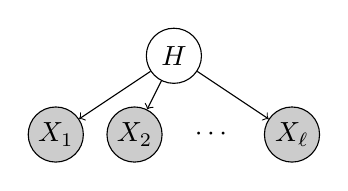
\begin{tikzpicture}
  [
    scale=1.0,
    observed/.style={circle,minimum size=0.7cm,inner sep=0mm,draw=black,fill=black!20},
    hidden/.style={circle,minimum size=0.7cm,inner sep=0mm,draw=black},
  ]
  \node [hidden,name=h] at ($(0,0)$) {$H$};
  \node [observed,name=x1] at ($(-1.5,-1)$) {$X_1$};
  \node [observed,name=x2] at ($(-0.5,-1)$) {$X_2$};
  \node at ($(0.5,-1)$) {$\dotsb$};
  \node [observed,name=xl] at ($(1.5,-1)$) {$X_\ell$};
  \draw [->] (h) to (x1);
  \draw [->] (h) to (x2);
  \draw [->] (h) to (xl);
\end{tikzpicture}}
\hfil\subfigure[Hidden Markov model]{\label{fig:hmm}
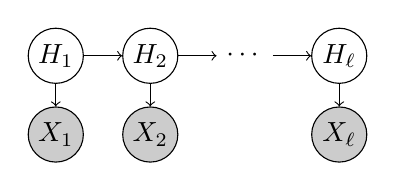
\begin{tikzpicture}
  [
    scale=1.0,
    observed/.style={circle,minimum size=0.7cm,inner sep=0mm,draw=black,fill=black!20},
    hidden/.style={circle,minimum size=0.7cm,inner sep=0mm,draw=black},
  ]
  \node [hidden,name=h1] at ($(-1.2,0)$) {$H_1$};
  \node [hidden,name=h2] at ($(0,0)$) {$H_2$};
  \node [name=hd] at ($(1.2,0)$) {$\dotsb$};
  \node [hidden,name=hl] at ($(2.4,0)$) {$H_\ell$};
  \node [observed,name=x1] at ($(-1.2,-1)$) {$X_1$};
  \node [observed,name=x2] at ($(0,-1)$) {$X_2$};
  \node [observed,name=xl] at ($(2.4,-1)$) {$X_\ell$};
  \draw [->] (h1) to (h2);
  \draw [->] (h2) to (hd);
  \draw [->] (hd) to (hl);
  \draw [->] (h1) to (x1);
  \draw [->] (h2) to (x2);
  \draw [->] (hl) to (xl);
\end{tikzpicture}}
\end{center}
\vspace{-5mm}
\caption{Examples of latent variable models.
}
\label{fig:graphical-model}
\vspace{-1mm}
\end{figure}

Multi-view latent variable models (\eg,~na\"ive Bayes models) are a
special class of Bayesian networks in which observed variables $X_1, X_2,
\ldots, X_\ell$ are conditionally independent given a latent variable $H$, and
the conditional distributions, $P(X_t|H)$, of the $X_t, t \in [\ell]$ given the hidden variable $H$ can be different. Two examples of latent variable models in this class can be found in~Figure~\ref{fig:graphical-model}. For simplicity of exposition, we now consider three random variables, $X_1, X_2$ and $X_3$ which are conditionally independent given $H$, and
\[
 P_j(X_t) \ :=\ P(X_t\, |\, H = j),\quad j \in [k],\ t \in \{1,2,3\}
\]
We first note that the distribution factorizes as follows
\begin{align}
P( X_t, X_{t'} )
\ & =\ \sum_{j=1}^k \pi_j \cdot P_j(X_t) \cdot P_j(X_{t'}),
\quad \{t,t'\} \subset \{1,2,3\} ,\ t \neq t' \label{eq:joint2} \\
P(X_1, X_2, X_3)
\ & =\ \sum_{j=1}^k \pi_j \cdot P_j(X_1) \cdot P_j(X_2) \cdot P_j(X_3). \label{eq:joint3}
\end{align}

\noindent {\bf Identifiability.} Allman et al. showed that, under mild conditions, finite mixture of nonparametric product distributions is identifiable. The multiview latent variable model in~\eq{eq:joint3} has the same form as  the finite mixture of nonparametric product distribution, and therefore we can adapt Allman's results to the current setting.
\begin{theorem}
  Let $P(X_1,X_2,X_3)$ be a multiview latent variable model of the form~\eq{eq:joint3}, such that for every $t \in \{1,2,3\}$, the distributions $\{P_j(X_t)\}_{j \in [k]}$ are linearly independent. Then, the set of parameters $\{\pi_j,P_j(X_t)\}_{j \in [k], t \in \{1, 2, 3\}}$ are strictly identifiable from $P(X_1,X_2,X_3)$, up to label swapping of the $j$ index.
\end{theorem}

\section{Kernel Embedding of Distributions}
\label{sec:embedding}

We begin by providing an overview of kernel embeddings of distributions, which are \emph{implicit} mappings of distributions into potentially \emph{infinite} dimensional feature spaces.\footnote{By ``implicit'', we mean that we do not need to explicitly construct the feature spaces, and the actual computations boil down to kernel matrix operations.} A \emph{reproducing kernel Hilbert space (RKHS)} $\Fcal$ on $\Omega$ with a kernel $k(x,x')$ is a Hilbert space of
functions $f:\Omega \mapsto \RR$ with inner product $\inner{\cdot}{\cdot}_{\Fcal}$. Its element $k(x,\cdot)$ satisfies the reproducing property:
$\inner{f(\cdot)}{k(x, \cdot)}_{\Fcal} = f(x)$, and consequently, $\inner{k(x,\cdot)}{k(x', \cdot)}_{\Fcal} = k(x,x')$,
meaning that we can view the evaluation of a function $f$ at any point $x\in\Omega$ as an inner product. Alternatively, $k(x,\cdot)$ can  be viewed as an implicit feature map $\phi(x)$ where $k(x,x')=\inner{\phi(x)}{\phi(x')}_{\Fcal}$.\footnote{For simplicity of notation, we use the same kernel for $y$,~\ie,~$k(y,y')=\inner{\phi(y)}{\phi(y')}_{\Fcal}$}
Popular kernel functions on $\RR^n$ include the polynomial kernel $k(x,x') =
(\inner{x}{x'}+c)^d$ and the Gaussian RBF kernel $k(x,x') = \exp(-\sigma
  \nbr{x-x'}^2)$. Kernel functions have also been defined on
graphs, time series, dynamical systems, images and other structured
objects~\citep{SchTsuVer04}. Thus the methodology presented below can  readily be generalized to a diverse range of data types as long as kernel functions are defined for them.

The kernel embedding approach represents a probability distribution by an element in the RKHS associated with a kernel function~\cite{SmoGreSonSch07,SriGreFukLanetal08},
\begin{align}
  \mu_{X} := \EE_{X} \sbr{\phi(X)} = \int_{\Omega} \phi(x) ~dP(x),~~\label{eq:embedding}
\end{align}
where the distribution is mapped to its expected feature map,~\ie,~to a point in a potentially infinite-dimensional and implicit feature space.
 The mean embedding $\mu_{X}$ has the property that the expectation of any RKHS function $f$ can be evaluated as an inner product in $\Fcal$,
$
  \inner{\mu_{X}}{f}_{\Fcal} := \EE_{X} [f(X)] \quad\forall f\in\Fcal.~~\label{eq:embedding2}
$

Kernel embeddings can be readily generalized to joint distributions of two or more variables using tensor product feature spaces. For instance, we can embed a joint distribution of two variables $X$ and $Y$ into a tensor product feature space $\Fcal\otimes \Fcal$ by
\begin{align}
    \Ccal_{XY} := \EE_{XY}[\phi(X)\otimes \phi(Y)] = \int_{\Omega \times \Omega} \phi(x) \otimes \phi(y)~d P(x,y)
\end{align}
where we assume for simplicity that the two variables share the same domain $\Omega$ and kernel $k$, and the tensor product features satisfy $\inner{\phi(x)\otimes \phi(y) }{\phi(x')\otimes \phi(y') }_{\Fcal\otimes \Fcal}=k(x,x')k(y,y')$.

As a special case, the marginal probability vector of a discrete variable $X$, and the probability table of the joint distribution of  discrete variables $X$ and $Y$, are both kernel embeddings. To see this, let $x,y\in \cbr{1,\ldots,N}$ and use Kronecker delta kernel $k(x,x') = \delta(x,x')$. The corresponding feature map $\phi(x)$ is then the standard basis of $e_{x}$ in $\RR^N$. Then
\begin{align}
    \rbr{
      \begin{array}{c}
         P(x = 1) \cr
         \vdots \cr
         P(x = N)
       \end{array}
    } = \EE_X[e_X] = \mu_X,~~~~
    \rbr{
        \begin{array}{ccc}
            & & \cr
            & P(x=s,y=t) & \cr
            & &
        \end{array}
    } = \EE_{XY}[e_X \otimes e_Y] = \Ccal_{XY}. \label{eq:jointprobabilitytable}
\end{align}

The joint embeddings can also be viewed as an uncentered cross-covariance operator $\Ccal_{XY}:\Fcal\mapsto \Fcal$ by the standard equivalence between a tensor product feature and a linear map.
That is, given two functions $f,g\in\Fcal$, their covariance can be computed by
$
    \EE_{XY}[f(X)g(Y)]=\inner{f}{\Ccal_{XY} g}_{\Fcal}
$
, or equivalently
$
\inner{f\otimes g}{\Ccal_{XY}}_{\Fcal\otimes\Fcal},
$
where in the former we view $\Ccal_{XY}$ as an operator while in the latter we view it as an element in tensor product space.
By analogy, $\Ccal_{XX} := \EE_X[\phi(X)\otimes \phi(X)]$ and $\Ccal_{XYZ} := \EE_{XYZ}[\phi(X)\otimes\phi(Y)\otimes \phi(Z)]$ can also be defined,
the latter of which can be regarded as a multi-linear operator from $\Fcal\otimes\Fcal\otimes\Fcal$ to $\RR$.
It will be clear from the context whether we use $\Ccal_{XY}$ as an operator between two spaces or as an element from a tensor product feature space.

Kernel embedding of distributions have both rich representational power and a well-behaved empirical estimate.
 First, the mapping is injective for characteristic kernels~\cite{SriGreFukLanetal08}. That is, if two distributions, $P(X)$ and $Q(Y)$, are different, they will be mapped to two distinct points in the feature space. Many commonly used kernels are characteristic, such as the Gaussian RBF kernel $\exp(-\sigma \|x - x'\|^2)$ and Laplace kernel $\exp(-\sigma \|x - x'\|)$, which implies that if we embed distributions using these kernels, the distance of the mappings in feature space will give us an indication whether two distributions are identical or not.
This intuition has been exploited to design  state-of-the-art two-sample tests~\cite{GreBorRasSchetal12} and  independence tests~\cite{GreFukTeoSonetal08}.

While we rarely have access to the true underlying distribution, $P(X)$,
we can readily estimate its embedding using a finite sample average. Given a sample $\Dcal_{X} = \cbr{x_1, \ldots, x_m}$ of size $m$ drawn~\iid~from $P(X)$, the empirical kernel embedding is
\begin{align}
    \hmu_{X} &= \frac{1}{m} \sum\nolimits_{i=1}^m \phi(x_i). \label{eq:empirical_embedding}
\end{align}
This empirical estimate converges to its population counterpart in RKHS norm, $\|\hmu_X - \mu_X \|_{\Fcal}$, with a rate of $O_p(m^{-\frac{1}{2}})$~\cite{SmoGreSonSch07}. We note that this rate is independent of the dimension of $X$, meaning that statistics based on kernel embeddings circumvent the curse of dimensionality.

Kernel embeddings of joint distributions inherit the previous two properties of general embeddings: injectivity and easy empirical estimation. Given $m$ pairs of training examples $\Dcal_{XY}=\cbr{(x_1,y_1),\ldots,(x_m,y_m)}$ drawn \iid~from $P(X,Y)$,
the covariance operator $\Ccal_{XY}$ can then be estimated as
\begin{align}
 \hCcal_{XY}=\frac{1}{m}\sum_{i=1}^m \phi(x_i) \otimes \phi(y_i). \label{eq:empirical_covariance}
\end{align}

By virtue of the kernel trick, most of the computation required for statistical inference using kernel embeddings can be reduced to the Gram matrix manipulation. The entries in the Gram matrix $K$ correspond to the kernel value between data points $x_i$ and $x_j$,~\ie,~$K_{ij} = k(x_i,x_j)$, and therefore its size is determined by the number of data points in the sample (similarly Gram matrix $G$ has entries $G_{ij}=k(y_i,y_j)$  ). The size of the Gram matrices is in general much smaller than the dimension of the feature spaces (which can be infinite). This enables efficient nonparametric methods using the kernel embedding representation. If the sample size is large, the computation in kernel embedding methods may be expensive. In this case, a popular solution is to use a low-rank approximation of the Gram matrix, such as incomplete Cholesky factorization~\cite{FinSch01}, which is known to work very effectively in reducing computational cost of kernel methods, while maintaining the approximation accuracy.

\noindent {\bf Relation between kernel embedding and the density function.} Basically kernel embeddings maps the density to a function in the RKHS. See Steinwardt and Vert.

\section{Kernel Embeddings of Conditional Distributions}
\label{sec:conditionalembedding}

The kernel embedding of a conditional distribution $P(Y|X)$ is defined as~\cite{SonHuaSmoFuk09}
\begin{align}
    \label{eq:conditionalembedding}
    \mu_{Y|x} :=\EE_{Y|x}[\phi(Y)] = \int_{\Omega} \phi(y)~dP(y|x).
\end{align}
Given this embedding, the conditional expectation of a function $g\in \Fcal$  can be computed as
$
    \label{eq:conditionalexpectation}
    \EE_{Y|x}[g(Y)] = \inner{g}{\mu_{Y|x}}_{\Fcal}.
$
This may be compared with the property of the mean embedding in the last section,
where the {\em unconditional} expectation of a function may be written as an inner product with the embedding.
Unlike the embeddings discussed in the previous section, an embedding of conditional distribution is not a single element in the RKHS, but will instead sweep out a family of
points in the RKHS, each indexed by a fixed value $x$ of the conditioning variable $X$. It is only
by fixing $X$ to a particular value $x$, that we will be able to obtain a single RKHS element, $\mu_{Y|x}\in\Fcal$. In other words, we need to define an operator, denoted as $\Ccal_{Y|X}$, which can take as input an $x$ and output an embedding. More specifically, we will
want it to satisfy
\begin{align}
    \label{eq:conditionalembeddingrequirement}
    \mu_{Y|x} = \Ccal_{Y|X} \phi(x).
\end{align}

Based on the relation between conditional expectation and covariance operators, Song et al.~\cite{SonHuaSmoFuk09} show that, under the assumption $\EE_{Y|\cdot} \sbr{g(Y)}\in\Fcal$,
\begin{align}
    \label{eq:conditionalembeddingoperator}
    \Ccal_{Y|X}:=\Ccal_{YX}\Ccal_{XX}^{-1},\quad\text{and hence}~\mu_{Y|x} = \Ccal_{YX} \Ccal_{XX}^{-1} \phi(x)
\end{align}
satisfy the requirement in~\eq{eq:conditionalembeddingrequirement}.
We remark that the assumption $\EE_{Y|\cdot} \sbr{g(Y)}\in\Fcal$ always holds for finite domains with characteristic kernels, but it is not necessarily true for continuous domains~\cite{FukBacJor04}. In the cases where the assumption does not hold,
we will use the expression $\Ccal_{YX}\Ccal_{XX}^{-1} \phi(x)$ as an approximation of the conditional mean $\mu_{Y|x}$.
In practice, the inversion of the operator can be replaced by the regularized inverse $(\Ccal_{XX}+\lambda I)^{-1}$.

The definition of the conditional embedding operator in~\eq{eq:conditionalembeddingoperator} is very general, and the conditional probability $P(Y|X)$ for discrete variables becomes a special case. For instance, if we use a Kronecker delta kernel and a construction similar to~\eq{eq:jointprobabilitytable}, we can obtain the conditional probability table by
\begin{align}
    \underbrace{\rbr{
        \begin{array}{ccc}
             &  &  \cr
            &  P(y=s|x=t) & \cr
            & &
        \end{array}
    }}_{\Ccal_{Y|X}}
    =
    \underbrace{
    \rbr{
        \begin{array}{ccc}
            & & \cr
            & P(y=s, x=t) & \cr
            & &
        \end{array}
    }}_{\Ccal_{YX}}
    \underbrace{
    \rbr{
        \begin{array}{ccc}
            P(x=1) & \ldots & 0 \cr
            \vdots &  \ddots & \vdots \cr
            0 & \ldots & P(x=N)
        \end{array}
    }^{\Large -1}}_{\Ccal_{XX}^{-1}}. \label{eq:conditionalprobabilitytable}
\end{align}
As a second example, let $Y$ from a general domain $\Omega$ while $X$ being discrete. In this case, there are $k$ different conditional distributions, $P(Y|x=t),\,t\in[k]$, one for each value of the discrete conditing variable $X$. Using Kronecker delta kernel for $X$, the conditional embedding operator is simply a column concatenation of the embeddings for each $P(Y|x)$,~\ie,
\begin{align}
  \Ccal_{Y|X} = \rbr{\mu_{Y|x=1},\ \mu_{Y|x=2},\ \ldots,\ \mu_{Y|x=k}}
\end{align}


Given a dataset $\Dcal_{XY}=\cbr{(x_1,y_1),\ldots,(x_m,y_m)}$ of size $m$ drawn~\iid~from $P(X,Y)$, we will estimate the conditional embedding operator as
\begin{align}
    & \widehat{\Ccal}_{Y|X} = \Phi (K + \lambda I)^{-1} \Upsilon^\top  \label{eq:embeddingoperatorestimator}
\end{align}
where $\Phi:=(\phi(y_1),\ldots,\phi(y_m))$ and $\Upsilon:=(\phi(x_1),\ldots,\phi(x_m))$ are implicitly formed feature matrix, and $K=\Upsilon^\top \Upsilon$ is the Gram matrix for samples from variable $X$. Furthermore, we need the additional regularization parameter $\lambda$ to avoid overfitting. Then $\hmu_{Y|x}=\widehat{\Ccal}_{Y|X}\phi(x)$ becomes a weighted sum of feature mapped data points from $Y$,
\begin{align}
    & \hmu_{Y|x} = \sum_{i=1}^m \beta_i(x) \phi(y_i) = \Phi \boldsymbol{\beta}(x) \quad \text{where}~ \label{eq:conditionalembeddingestimator}\\
    & \boldsymbol{\beta}(x) = \rbr{\beta_1(x), \ldots, \beta_m(x)}^\top = (K + \lambda I)^{-1} K_{: x}, \nonumber
\end{align}
and $K_{: x}=(k(x,X_1),\ldots,k(x,X_m))^\top$.
The empirical estimator of the conditional embedding
is similar to the estimator of the ordinary embedding from
equation~\eq{eq:embedding}. The difference
is that, instead of applying uniform weights $\frac{1}{m}$,
the former applies {\em non-uniform} weights, $\beta_i(x)$, on
observations which are, in turn, determined by the value $x$ of the conditioning
variable. These non-uniform weights reflect the effects of
conditioning on the embeddings. It is also shown that this empirical estimate converges to its population counterpart in RKHS norm, $\nbr{\hmu_{Y|x} - \mu_{Y|x}}_{\Fcal}$, with rate of $O_p(m^{-\frac{1}{4}})$ if one decreases the regularization $\lambda$ with rate $O(m^{-\frac{1}{2}})$.

\section{Kernel Embedding of Multiview Latent Variable Models}

Then we can embedding into RKHS the second and third order marginal distribution of the observed variables in the multiview latent variable models in~\eq{eq:joint2} and~\eq{eq:joint3}. These kernel embeddings will also factorize according the conditional independence structure of the underlying model. More specifically,
\begin{align*}
  \Ccal_{X_1,X_2,X_3}
  = \EE_{X_1,X_2,X_3}[\phi(X_1)\otimes \phi(X_2) \otimes \phi(X_3)]
\end{align*}
Making use of the distribution factorization of the model, we have that
\begin{align*}
  \Ccal_{X_1,X_2,X_3} =
  \sum_{j=1}^k \pi_j \cdot \EE_{X_1| H=j}[\phi(X_1)]\otimes \EE_{X_2|H=j} [\phi(X_2)] \otimes \EE_{X_3|H=j}[\phi(X_3)]
\end{align*}
where $\mu_{X_t|j}:=\EE_{X_t| H=j}[\phi(X_t)] = \int_{\Omega} \phi(X_t)\, d P(X_t|H=j)$ is the
the conditional embedding of the observed variable $X_t$ given latent variable $H=j$.
Then we can express the embedding $\Ccal_{X_1,X_2,X_3}$ as a sum of outer product of conditional embeddings,~\ie,
\begin{align*}
  \Ccal_{X_1,X_2,X_3}
  = \sum_{j=1}^k \pi_j \cdot \mu_{X_1|j} \otimes \mu_{X_2|j} \otimes \mu_{X_3|j}
\end{align*}
Similarly, for the joint distribution of the two observed variable in~\eq{eq:joint2}, we have
\begin{align*}
  \Ccal_{X_t,X_{t'}}
  = \sum_{j=1}^k \pi_j \cdot \mu_{X_t|j} \otimes \mu_{X_{t'}|j},\quad \{t,t'\} \subset \{1,2,3\},\ t\neq t'
\end{align*}

% \section{Whitening with Three Different Views}

% \begin{itemize}
% 	\item $\widetilde{\Ccal}_{12} = \Ccal_{12} \Ucal_2^\top$; $\widetilde{\Ccal}_{13} = \Ccal_{13} \Ucal_3^\top$; $\widetilde{\Ccal}_{23} = \Ucal_{2} \Ccal_{23} \Ucal_3^\top$
% 	\item $\widetilde{\Ccal}_{11} = \widetilde{\Ccal}_{12} (\widetilde{\Ccal}_{32})^{-1} \widetilde{\Ccal}_{31}^\top = \widetilde{\Ucal}_1 \widetilde{\Scal}_1 \widetilde{\Ucal}_1^\top$
% 	\item $\widetilde{\Tcal} = \Ccal_{123} \bullet_1 (\widetilde{\Ucal}_1 \widetilde{\Scal}_1^{-1/2})^\top  \bullet_2 (\widetilde{\Ucal}_2 \widetilde{\Scal}_2^{-1/2})^\top \bullet_3 (\widetilde{\Ucal}_3 \widetilde{\Scal}_3^{-1/2})^\top$
% \end{itemize}

For simplicity of exposition, assume that $\mu_{X_t|j} = \mu_{X_{t'}|j}$ for $t\neq t'$. Then the parameters, $\{\pi_j, \mu_{X_t|j}\}_{j \in [k]}$, of the multiview latent variable model can be recovered from $\Ccal_{X_t,X_{t'}}$ and $\Ccal_{X_1,X_2,X_3}$ using the following simple algorithm
\begin{enumerate}
  \item Singular value decomposition for $\Ccal_{X_t,X_{t'}}$,
    $$\Ccal_{X_t,X_{t'}} = U\, S\,\, V^\top$$
  \item Let the leading $k$ eigen-vectors corresponding to the largest $k$ eigen-value be $U_k$, and the corresponding submatrix of $S$ containing these eigen-values be $S_k$.
  \item Whiten the embedding $\Ccal_{X_1,X_2,X_3}$,
    $$\Tcal := \Ccal_{X_1,X_2,X_3} \times_1 (S_k^{-1/2}U_k^\top) \times_2 (S_k^{-1/2}U_k^\top) \times_3 (S_k^{-1/2}U_k^\top)$$
    where $\times_i$ denotes mode-$i$ tensor-matrix multiplication.
  \item Find the leading $k$ tensor eigen-vectors $V_k$ for $\Tcal$ using tensor power method.
  \item Recover the embedding $\mu_{X_t|j}$ by
    $$ (\mu_{X_t|j})_{j \in [k]}  = (S_k^{-1/2}U_k^\top)^\dagger V_k $$
\end{enumerate}

\section{Kernel Algorithm}

Given $m$ observation $\Dcal_{X_1,X_2,X_3}=\{(x_1^i,x_2^i,x_3^i)\}_{i \in [m]}$ drawn~\iid~from a multi-view latent variable model $P(X_1,X_2,X_3)$, we now design a kernel algorithm to estimate the latent parameters from data. Although the empirical kernel embedding has infinite dimensions, we can carry out the decomposition using just the kernel matrices.

First, we will perform a kernel singular value decomposition of the empirical estimate of $\widehat \Ccal_{X_t,X_{t'}}:= \frac{1}{m} \sum_{i=1}^m \phi(x_t^i) \otimes \phi(x_{t'}^i)$. Denote the implicitly formed feature matrix for variable $X_t$ by $\Phi := (\phi(x_t^1),  \phi(x_t^2), \ldots, \phi(x_t^m))$, and that for variable $X_{t'}$ by $\Psi := (\phi(x_{t'}^1), \phi(x_{t'}^2), \ldots, \phi(x_{t'}^m))$ respectively. And the corresponding kernel matrix be $K = \Phi^\top \Phi$ and $L = \Psi^\top \Psi$. Using the feature matrice, $\Ccal_{X_t,X_{t'}}$ can be expressed as
$$
	\Ccal_{X_t,X_{t'}} = \frac{1}{m} \Phi \Psi^\top.
$$
Its leading $k$ singular vector $U_k = (u_1,\ldots,u_k)$ will lie in the span of the column of  $\Phi$,~\ie,~$U_k = \Phi (\betab_1,\ldots,\betab_k)$ where $\betab \in \RR^m$. Then we can transform the singular value decomposition problem for an infinite dimensional matrix to a generalized eigenvalue problem involving kernel matrices,
$$
	\Ccal_{X_t,X_{t'}} \Ccal_{X_t,X_{t'}}^\top u = \lambda\;u
	\quad \Leftrightarrow \quad
	\frac{1}{m^2}\Phi \Psi^\top \Psi \Phi^\top \Phi \betab = \lambda\,\Phi \betab
	\quad \Leftrightarrow \quad
	\frac{1}{n^2} K L K \betab = \lambda\,K \betab.
$$
Let the Cholesky decomposition of $K$ be $R^\top R$, then the generalized eigenvalue decomposition problem can be solved by redefining $\widetilde{\betab}=R\betab$, and solving an ordinary eigenvalue problem
\begin{align}
 \frac{1}{n^2} R L R^\top \widetilde{\betab} = \lambda\, \widetilde{\betab},~~\text{and obtain}~\betab = R^{\dagger} \widetilde{\betab}.
\end{align}
The resulting singular vectors satisfy $u_j^\top u_{j'} = \betab_l^\top \Phi^\top \Phi_1 \betab_{j'} =  \betab_{j}^\top K  \betab_{j'} =  \widetilde{\betab}_{j}^\top \widetilde{\betab}_{j'}=\delta_{jj'}$.

\begin{algorithm}[t!]
\caption{KernelSVD($K$, $L$, $k$)}
% 	\textbf{In}: Two kernel matrices $K$ and $L$, and desired rank $r$ \\
	\textbf{Out}: $S_k$ and $(\betab_1,\ldots,\betab_k)$\\[-0.4cm]
  \begin{algorithmic}[1]
    \STATE Perform Cholesky decomposition:\ $K=R^\top R$
    \STATE Solve eigen-decomposition problem:\ $\frac{1}{m^2} R L R^\top \widetilde{\betab} = \lambda\,\widetilde{\betab}$
		\STATE Let the $k$ leading eigen-values be:\ $S_k = \diag(\lambda_1,\ldots,\lambda_k)$
		\STATE Let the corresponding $k$ leading eigen-vectors be:\ $(\widetilde{\betab}_1,\ldots,\widetilde{\betab}_k)$
    \STATE Compute:\ $(\betab_1,\ldots,\betab_k) = R^\dagger (\widetilde{\betab}_1,\ldots,\widetilde{\betab}_k)$
% 		, and reorgnaize $(\thetab^1,\ldots,\thetab^n)^\top = (\betab_1,\ldots,\betab_k)$
  \end{algorithmic}
  \label{alg:svd}
\end{algorithm}

Second, we will whiten the empirical embedding $\widehat \Ccal_{X_1,X_2,X_3}:=\frac{1}{m}\sum_{i=1}^m \phi(x_1^i) \otimes \phi(x_2^i) \otimes \phi(x_3^i)$ by
\begin{align}
	\widehat \Tcal := \frac{1}{m}\sum_{i=1}^m \widetilde K_{:x_1^i} \otimes \widetilde K_{:x_2^i} \otimes \widetilde K_{:x_3^i} \quad \in \quad \RR^{k\times k \times k},
\end{align}
where $\widetilde K_{:x_t^i}$ is related to a column of the kernel matrix $K$
$$
	K_{:x_t^i} := S_k^{-1/2} (\betab_1,\ldots,\betab_k)^\top \Phi^\top \phi(x_t^i).
$$

Next, we run tensor power method on the finite dimension tensor $\widehat \Tcal$ to obtain its leading $k$ eigen-vectors $V_k$. Last, the estimate for the latent parameters is given by
\begin{align}
	(\mu_{X_t|j})_{j\in[k]} = \Phi (\betab_1,\ldots,\betab_k) S_k^{1/2} V_k
\end{align}

\section{Statistical Analysis}

Concentration results for the singular value decomposition of empirical operators.

\begin{theorem} Let $\kappa:=\sup_{x \in \Omega} k(x,x)$, and $\| \cdot\|_{HS}$ be the Hilbert-Schdmit norm, we have
\begin{eqnarray}
	\PP \cbr{ \nbr{\Ccal_{X_t,X_{t'}} - \widehat \Ccal_{X_t,X_{t'}}}_{HS} \leqslant \frac{2\sqrt{2}\kappa \sqrt{\delta}}{\sqrt{n}} } \geqslant 1-2\exp(-\delta). \label{eq:operator_concentration}
\end{eqnarray}
\end{theorem}

\begin{proof}
We will use similar arguments as in~\cite{RosBelVit2010} which deals with symmetric operator. Let $\xi_{i}$ be defined as
\begin{eqnarray}
\xi_{i}\, =\, \phi(x_t^i) \otimes \phi(x_{t'}^i) - \Ccal_{X_t,X_{t'}}.
\end{eqnarray}
It is easy to see that $\mathbb{E}[\xi_{i}] = 0$. Further, we have
\begin{eqnarray}
	\sup_{x_t,x_{t'}} \nbr{\phi(x_t) \otimes \phi(x_{t'})}^{2}_{HS} \leqslant \kappa^{2},
\end{eqnarray}
which implies that $\nbr{\Ccal_{X_t,X_{t'}}}_{HS} \leqslant \kappa$, and $\nbr{\xi_i}_{HS} \leqslant 2 \kappa$. The result then follows from the Hoeffding's inequality in Hilbert space.
\end{proof}


Use analysis for tensor paper and then concentration inequality for Hilbert space embeddings.

\section{Intepretation with Parametric Family}

For interpretable results, we can project the nonparametric representation to parametric family of distributions (\eg,~exponential families) as post-processing.

\bibliographystyle{unsrt}
\bibliography{../../../newbibfile/bibfile} % L
% \bibliography{../../../../newbibfile/bibfile} % L

\end{document}

%%%%%%%%%%%%%%%%%%%%%%%%%%%%%%%%%%
%%%%%%%%%%%%%%%%%%%%%%%%%%%%%%%%%%
%%%%%%%%%%%%%%%%%%%%%%%%%%%%%%%%%%


